% -*- fill-column: 85; -*-
%!TEX root = ../dissertation.tex
\section{Accelerator Silos}
\label{s:silo}

\begin{figure}[!t]
	\centering
	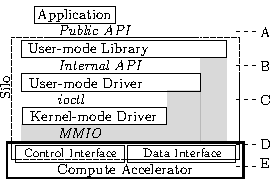
\includegraphics[width=.78\linewidth]{ava/images/silo.pdf}
	\caption{An accelerator silo.
		The public API and the interfaces with striped backgrounds are interposition candidates.
		All interfaces with backgrounds are proprietary and subject to change.
        }
	\label{fig:silo}
\end{figure}

Accelerator stacks
compose layered components that include a user-mode library to support an
API framework and a driver to manage the device.
Vendors are incentived to use proprietary interfaces and protocols between layers to preserve forward compatibility,
and to use kernel-bypass communication techniques to eliminate OS overheads.
However, interposing opaque, frequently-changing interfaces communicating with memory
mapped command rings is \emph{impractical} because it requires inefficient techniques and
yields solutions that sacrifice compatibility.
Consequently, accelerator stacks are effectively \emph{silos}
(Figure~\ref{fig:silo}), whose intermediate layers
\emph{cannot be practically separated} to virtualize the device.

\paragraphbe{Current support.} Most current hardware accelerators feature some
hardware support for virtualization: primarily for process-level address-space
separation, and in a small handful of cases, SR-IOV.
A central premise of this paper is that hardware support for process-level
isolation \emph{could} suffice to support hypervisor-level virtualization as
well, but the siloed structure of current accelerator stacks prevents it.

\begin{figure*}[!!thp!]
    \centering
    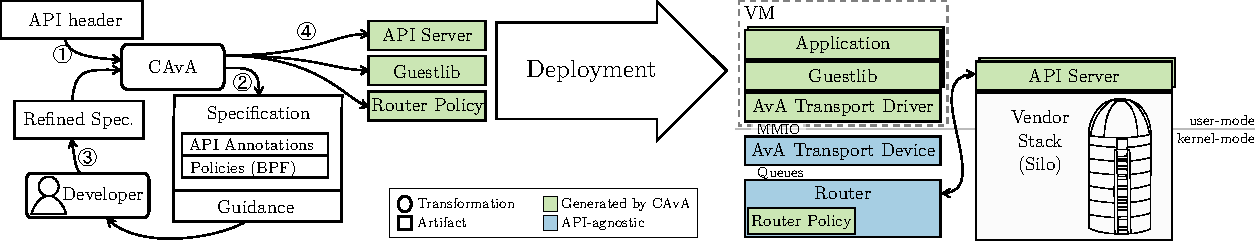
\includegraphics[width=\textwidth]{ava/images/overview.pdf}
    \caption{Overview of \model.}
    \label{fig:overview}
    \vspace*{-1em}
\end{figure*}


For accelerator silos, the \emph{only} stable and
efficiently interposable interface is the framework API, so
we focus on techniques to recover or compensate virtualization properties lost by
API remoting: interposition and compatibility.
Interposition can be recovered by using hypervisor-managed forwarding transport,
creating a central interface at which to enforce resource management policies.
\Model uses a novel technique called \emph{\noveltechnique (\novtechabbrv)} to achieve this.
\novtechabbrv presents guest VMs with an abstract virtual device with MMIO Base Address Registers (BAR), but this device is \emph{not a virtual accelerator}, but an endpoint that
routes communication through the hypervisor.

Using hypervisor-managed transport recovers interposition, but complicates compatibility and introduces engineering effort:
\novtechabbrv requires custom guest libraries, guest drivers, and API servers for each OS and API, and API-specific resource-management code in the hypervisor.
\model mitigates this with automated construction (\S\ref{s:api}).
Automatically generating code to implement \novtechabbrv components presents several challenges which
follow from the need to specify API semantics and policies for which
existing Interface Description Languages (IDLs)~\cite{Lamb1987,MSIDL} are not applicable.
\Model uses a new DSL called \speclang, a compiler called \compiler, and device-agnostic transport components to address these challenges.

% because semantic information %and resource management
%specifications required for virtualization are beyond the scope of existing IDLs.
%sharing policy specifications that are beyond the scope of IDLs.
%Designing efficient and flexible transport layers, and enforcing resource-sharing policies at the transport layer where semantic %information about the underlying device resources is not readily available are additional challenges.
% In subsequent sections, we show how
